\documentclass[a4paper,12pt]{refart}

\usepackage[spanish]{babel}
\usepackage[utf8]{inputenc}
\usepackage[T1]{fontenc} % LY1 also works

%% Font settings suggested by fbb documentation.
\usepackage{textcomp} % to get the right copyright, etc.
\usepackage[lining,tabular]{fbb} % so math uses tabular lining figures
\usepackage[scaled=.95,type1]{cabin} % sans serif in style of Gill Sans
\usepackage[varqu,varl]{zi4}% inconsolata typewriter
\useosf % change normal text to use proportional oldstyle figures
%\usetosf would provide tabular oldstyle figures in text
%\usepackage{avant}
\usepackage{mathptmx}

\usepackage{microtype}

\usepackage{float}

\usepackage{graphicx}
\usepackage[export]{adjustbox}
\usepackage{enumitem}
\setlist{leftmargin=*}
\usepackage{listings}
\usepackage{framed}
\usepackage{etoolbox}
%\AtBeginEnvironment{leftbar}{\sffamily\small}

\usepackage[os=win]{menukeys}
\renewmenumacro{\menu}[>]{roundedmenus} % default: menus
\renewmenumacro{\directory}{pathswithfolder} % default: paths
\renewmenumacro{\keys}[+]{shadowedroundedkeys} % default: roundedkeys

\usetikzlibrary{chains,arrows,shapes,positioning}
\usepackage{hyperref}

\lstset{
backgroundcolor=\color{black},
basicstyle=\ttfamily\scriptsize\fontsize{10}{10}\color{green},xleftmargin=3em,xrightmargin=3em,frame=single,
breaklines=true,
language=bash,
showstringspaces=false
}

\newcommand\commandList{\textit{lista de comandos}}
\newcommand\commandEditor{\textit{editor de comandos}}
\newcommand\interfaceEditor{\textit{editor de interfaces}}
\newcommand\tarpuqJIGsw{\textbf{Tarpuq JIGsw}}
\renewcommand\abstractname{Introducción}

%\definecolor{tqblue}{RGB}{0,161,228}
\definecolor{tqblue}{RGB}{255,255,255}
\definecolor{forestgreen(web)}{rgb}{0.13, 0.55, 0.13}

\usepackage{fancyhdr}
\usepackage{tikz}
\pagestyle{fancy}
\fancyhf{}
\fancyhead[C]{%
	\begin{tikzpicture}[overlay, remember picture]%
    \fill[tqblue] (current page.north west) rectangle ($(current page.north east)+(0,-1in)$);
    \node[anchor=north east, text=black, font=\Large\scshape, minimum size=1in, inner xsep=15mm] at (current page.north east) {Tarpuq JIGsw - Manual de Usuario};
    \node[anchor=north west, minimum size=1in, inner xsep=15mm] at (current page.north west) {
\includegraphics[scale=.2]{images/LogoNuevo_color}};
    %node[minimum width=\x2-\x1, minimum height=2cm, draw, rectangle, fill=blue!20, anchor=north west, align=left, text width=\x2-\x1] at ($(current page.north west)$) {\Large\bfseries \quad #1};
	\end{tikzpicture}
}
\fancyfoot[CO,CE]{
    \begin{tikzpicture}[overlay, remember picture]%
    \fill[tqblue] (current page.south west) rectangle ($(current page.south east)+(0,.5in)$);
	\node[anchor=south, text=forestgreen(web), inner ysep=10mm] at (current page.south) {Por favor considera el ambiente antes de imprimir};
	\node[anchor=south east, text=black, inner ysep=10mm, inner xsep=10mm] at (current page.south east) {Copia Controlada};
    \node[anchor=south west, text=black, font=\Large, minimum size=.5in] at (current page.south west) {\thepage};
    \node[anchor=south, text=black, font=\large, minimum size=.5in] at (current page.south) {\leftmark};
    \node[anchor=south east, text=black, font=\large, minimum size=.5in, inner xsep=5mm] at (current page.south east) {\today};
	\end{tikzpicture}
}
\setlength{\headheight}{12pt}
\settextfraction{0.8}

\usepackage{draftwatermark}
\SetWatermarkText{Confidencial}
\SetWatermarkScale{0.7}
\SetWatermarkColor[rgb]{0.95,0.95,0.95}

\title{Tarpuq JIGsw}
\author{Galo Guzmán (\url{gguzman@tarpuq-ems.com}) }

\makeatletter         
\def\@maketitle{%
	\newpage
	\null
	\longthickrule\vskip1.5em%
	\let \footnote \thanks
	\begin{flushright}%
	{
\includegraphics[scale=.45]{images/LogoNuevo_color} \par}%
	{\Huge\bfseries \@title \par}%
	{\Huge\bfseries Manual de Usuario \par}%
	\end{flushright}
	\vskip1.5em\longthickrule\vskip1.5em%
	{\normalsize
		\lineskip .5em%
		\begin{flushright}%
		{\slshape\@author\par}
		\vskip 1em%
		{\@date}%
		\end{flushright}\par}%
	\vskip 1.5em
}
\makeatother

\makeatletter
\renewenvironment{table}%
  {\renewcommand\familydefault\sfdefault
   \@float{table}}
  {\end@float}
\makeatother

\begin{document}
\maketitle

\begin{abstract}
\tarpuqJIGsw\ es una herramienta de automatización para el proceso de pruebas en producción de cualquier dispositivo desarrollado por Tarpuq Cia. Ltda.
Permite crear un perfil de pruebas, el cual será específico para cada producto. El perfil consta de un conjunto de comandos que permiten interactuar con los diferentes dispositivos de pruebas, programación, así como con el DUT (Device Under Test) a través de diferentes interfaces (p.e. UART, Pickit).
\end{abstract}

Documento de referencia No. xxxxxxxxxxxxxxxxx

\newpage

\tableofcontents

\section{Requerimientos del sistema}
\begin{itemize}
\item Computadora con procesador x86-64.
\item Sistema operativo Ubuntu 18.04.
\item Tener instalado MPLAB X IDE 5.10 o superior (recomendado instalar únicamente MPLAB X IPE).
\item Tener acceso a un servidor con base de datos MySQL (de preferencia que sea remoto, para tener acceso desde la aplicación de reportes).
\item Conexión de red.
\end{itemize}

\section{Instalación}
La instalación del programa de pruebas se puede llevar a cabo de 2 formas.

\paragraph{Método 1:}
Abriendo el paquete de instalación \directory{tarpuqJIGsw.deb} desde un navegador de archivos (Nautilus por defecto en Ubuntu). Luego dar clic en \keys{Instalar}.

\begin{figure}[H]\centering
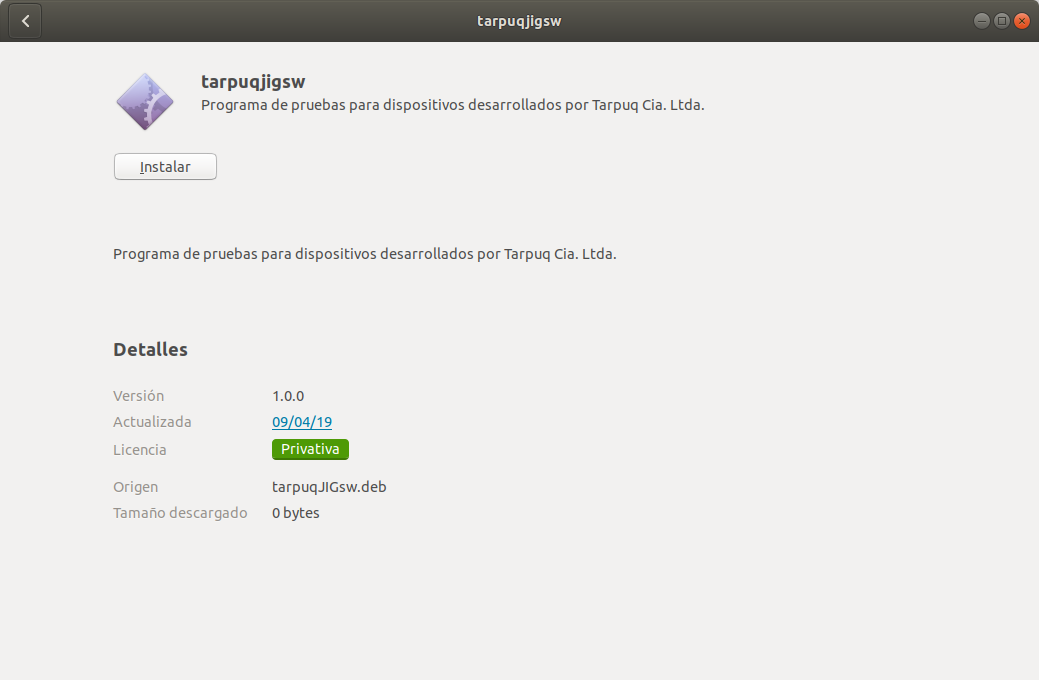
\includegraphics[width=\textwidth, frame]{images/install_ubuntu}
\caption{Instalación de \tarpuqJIGsw{} en Ubuntu}
\label{fig:installDeb}
\end{figure}

\paragraph{Método 2:}
Ejecutando el comando ``sudo dpkg -i tarpuqJIGsw.deb'' en una terminal.

\subsection{Configuración del sistema}\label{ref:sysConfig}
Para el correcto funcionamiento de \tarpuqJIGsw\, es necesario dar permisos del sistema a los dispositivos seriales y al programador PicKit. Esto se realiza de la siguiente forma:

\begin{enumerate}
\item Abrir una terminal de comandos.

\item Agregar al usuario principal al grupo dialout, ejecutando el siguiente comando:

\begin{lstlisting}
$sudo adduser $USER dialout
\end{lstlisting}

\item Cambiar los permisos para udev requeridos por MPLAB ejecutando el siguiente comando:
\begin{lstlisting}
$sudo systemctl edit systemd-udevd
\end{lstlisting}

Se abrirá un editor de texto con un archivo llamado ``override'' en el que es necesario agregar las siguientes líneas:

\begin{lstlisting}
[Service]
IPAddressAllow=localhost
\end{lstlisting}

Guardar los cambios y salir.

\item Dar los permisos para el PicKit en el archivo:
\\
\directory{/etc/udev/rules.d/z010\_mchp\_tools.rules}
\\
agregando la opción GROUP=``plugdev'' al final de las líneas de configuración, de la siguiente forma:

\begin{lstlisting}
ATTR{idVendor}=="04d8", ATTR{idProduct}=="8???", MODE="666", RUN+="%E{hotplugscript} add", GROUP="plugdev"
ATTR{idVendor}=="04d8", ATTR{idProduct}=="9???", MODE="666", RUN+="%E{hotplugscript} add", GROUP="plugdev"
ATTR{idVendor}=="04d8", ATTR{idProduct}=="a0??", MODE="666", RUN+="%E{hotplugscript} add", GROUP="plugdev"
ATTR{idVendor}=="04d8", ATTR{idProduct}=="00e0", MODE="666", RUN+="%E{hotplugscript} add", GROUP="plugdev"
ATTR{idVendor}=="04d8", ATTR{idProduct}=="00e1", MODE="666", RUN+="%E{hotplugscript} add", GROUP="plugdev"
ATTR{idVendor}=="03eb", ATTR{idProduct}!="6124", MODE="666", RUN+="%E{hotplugscript} add", GROUP="plugdev"
\end{lstlisting}

\item Agregar la ruta de Java JRE en el archivo \directory{ipecmd.sh}, el cual está en la ubicación:
\\
\directory{/opt/microchip/mplabx/vX.YY/mplab\_platform/\\
mplab\_ipe/ipecmd.sh}
\\
donde X.YY es la versión de MPLAB X que se encuentra instalada. El archivo contiene una línea que por defecto viene con la siguiente información:

\begin{lstlisting}
#jdkhome=/path/to/java
\end{lstlisting}

Hay que cambiar esta línea agregando la ruta de Java JRE que viene incluido con la instalación de MPLAB X. Esta puede ser copiada desde el archivo:
\\
\directory{/opt/microchip/mplabx/vX.YY/mplab\_platform/etc/\\
mplab\_ipe.conf}

\begin{lstlisting}
.
.
.

# Default location of JDK:
# (set by installer or commented out if launcher should decide)
#
# It can be overridden on command line by using --jdkhome <dir>
# Be careful when changing jdkhome.
# There are two NetBeans launchers for Windows (32-bit and 64-bit) and
# installer points to one of those in the NetBeans application shortcut 
# based on the Java version selected at installation time.
#
jdkhome="/opt/microchip/mplabx/v5.10/sys/java/jre1.8.0_181"
.
.
.
\end{lstlisting}

Solo debemos copiar la línea que contiene la ruta (jdkhome), al archivo ipecmd.sh.

\item Es necesario reiniciar la sesión de usuario para que todos los cambios tengan efecto.
 
\end{enumerate}

\subsection{Configuración del acceso a la base de datos}
En la versión actual esto se realiza editando el archivo de configuración del programa, el cual se crea al momento de la instalación en la ubicación por defecto:
\\
\directory{/usr/local/etc/tarpuqJIGsw.json}

Por defecto el archivo contiene la siguiente configuración:
\begin{lstlisting}
{
    "database":{
        "hostName":"DIR.IP.DEL.SERVIDOR",
        "databaseName":"NOMBRE_BASE_DE_DATOS",
        "userName":"tarpuqJIGsw",
        "password":"PASSWORD"
    },
    "api":{
        "hostName":"xxx.xxx.xxx.xxx",
        "userName":"admin",
        "password":"admin",
        "port":8080
    }
}
\end{lstlisting}

Para apuntar a otro servidor es necesario cambiar los parámetros del campo \textbf{database}.

\section{Interfaz de usuario}
\subsection{Ventana principal}
\tarpuqJIGsw\ tiene una interfaz de usuario que busca ser clara y sencilla para su manejo por parte del usuario final (operador).

\begin{figure}[hbt!]\centering
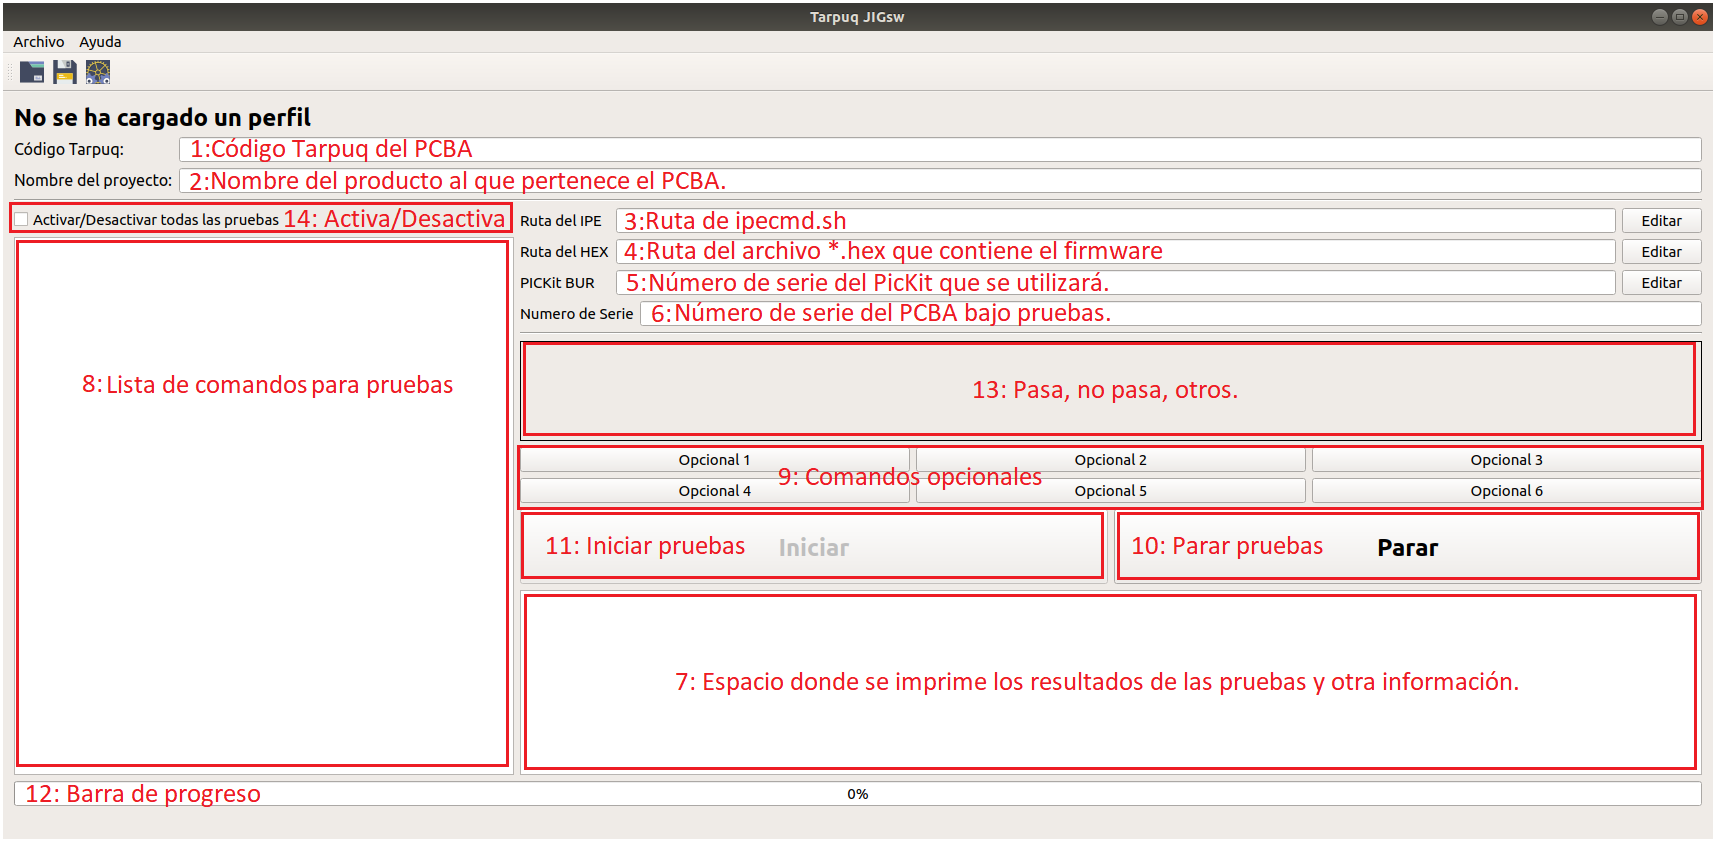
\includegraphics[width=\textwidth, frame]{images/main_new_description} 
\caption{Pantalla principal}
\label{fig:mainDescription}
\end{figure}

En la figura \ref{fig:mainDescription} podemos ver los diferentes segmentos que componen la \textit{ventana principal}. A continuación se detalla cada segmento de la figura:

\begin{enumerate}
\item \textbf{Código:} Es el código interno de Tarpuq asignado al PCBA bajo pruebas.
\item \textbf{Producto:} Es el nombre del producto al que pertenece el PCBA bajo pruebas, p.e. qiblí, medidores, etc.
\item \textbf{Ruta del IPE:} Ruta donde se encuentra la aplicación de control del PicKit, llamado ipecmd.sh. En la sección \ref{ref:sysConfig} del manual, podemos encontrar la ubicación por defecto.
\item \textbf{Ruta del HEX:} Ruta donde se encuentra el archivo compilado que contiene el firmware que va a ser programado en el PCBA bajo pruebas.
\item \textbf{PICKit BUR:} Cada PicKit tiene su BUR propio, es su número de serie, y es necesario para poder interactuar con el programador. Está ubicado en la etiqueta posterior del PicKit, o en su defecto puede ser leído con MPLAB IDE o MPLAB IPE.
\item \textbf{Número de serie:} Cada PCBA tiene su número de serie asignado en producción. Para iniciar las pruebas es necesario agregar éste número.
\item \textbf{Consola:} Las pruebas van entregando información mientras se van ejecutando. Esta información se muestra en este espacio y es personalizable (como se verá posteriormente), entregando mensajes para pruebas correctas o con error.
\item \textbf{Lista de comandos:} Las pruebas que serán realizadas, son ejecutadas como comandos. Estos comandos se muestran en este espacio, organizados en una tabla. La secuencia de ejecución respeta el orden en el que están ubicados los comandos en la tabla.
\item \textbf{Comandos opcionales:} Posteriormente se dotará a la aplicación de la capacidad de enviar comandos a ciertos dispositivos, en cualquier instante.
\item \textbf{Parar:} Detiene las pruebas al instante.
\item \textbf{Iniciar:} Inicia la secuencia de pruebas.
\item \textbf{Barra de progreso:} Indica el progreso de las pruebas.
\item \textbf{Cuadro de mensajes:} Muestra un mensaje de Pasa en fondo verde cuando las pruebas fueron exitosas. No pasa en fondo rojo cuando se ha producido una prueba fallida. Y varios mensajes del programa.
\item \textbf{Activar/Desactivar pruebas:} Activa o desactiva todas las pruebas disponibles en la tabla de pruebas.
\end{enumerate}

\subsubsection{Barra de herramientas}
El programa consta también de una barra de herramientas mostrado en la figura \ref{fig:toolbar}, con las opciones de Abrir, Guardar y Configuraciones respectivamente.

\begin{figure}[hbt!]\centering

\includegraphics[scale=1]{images/toolbar} 
\caption{Barra de herramientas}
\label{fig:toolbar}
\end{figure}

\begin{leftbar}
La opción de Configuraciones se encuentra en desarrollo, por lo que estará disponible en versiones futuras.
\end{leftbar}

\subsubsection{Lista de comandos} \label{ref:commandList}
Uno de los elementos más importantes de la interfaz principal de usuario, es la \commandList\, por lo que es necesario detallar este elemento.

La \commandList\ es una herramienta que permite mostrar y manipular los comandos del perfil de prueba. Se carga con la información de las pruebas (comandos) al momento de abrir un perfil.

\begin{figure}[hbt!]\centering
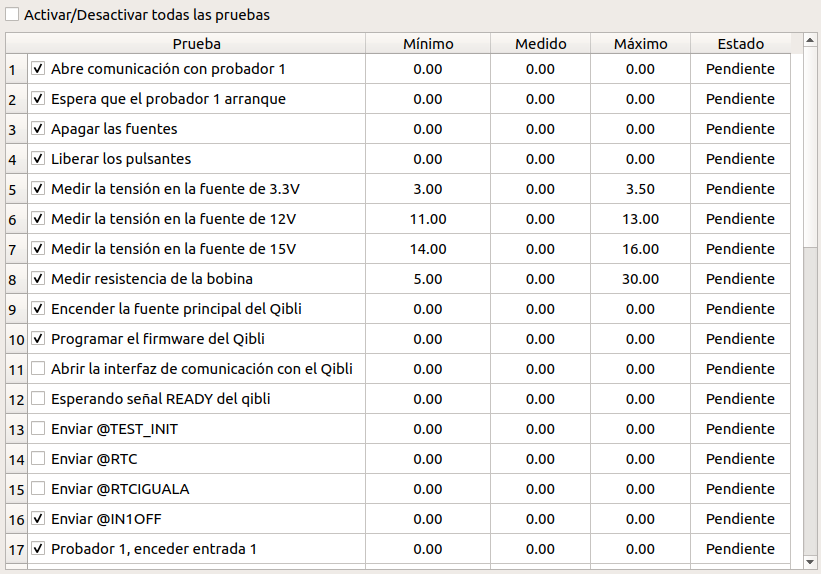
\includegraphics[width=\textwidth, frame]{images/main_commandList}
\caption{Lista de comandos}
\label{fig:commandList}
\end{figure}

En la \commandList\ mostrada en la figura \ref{fig:commandList} se puede identificar 5 columnas, las cuales son:

\begin{itemize}
\item \textbf{Prueba:} Breve descripción de lo que hace la prueba.
\item \textbf{Mínimo:} Umbral mínimo que puede tener una medición.
\item \textbf{Medido:} Es el valor medido en la prueba.
\item \textbf{Máximo:} Umbral máximo que puede tener una medición.
\item \textbf{Estado:} Muestra un mensaje del estado actual de la prueba, el cual puede ser:
	\begin{itemize}
	\item \textbf{Pendiente:} indica que la prueba esta en espera.
	\item \textbf{Demora:} la prueba está ejecutando una demora.
	\item \textbf{En ejecución:} esta prueba esta ejecutándose en este instante.
	\item \textbf{Salta:} esta prueba no se ejecuta, salta al siguiente comando.
	\item \textbf{Ok:} la prueba fue exitosa.
	\item \textbf{Error:} la prueba falló.
	\end{itemize}
\end{itemize}

Los comandos pueden ser alterados desde la \commandList{}. Se pueden crear nuevos comandos, pueden ser reubicados, eliminados, editados, duplicados. Para esto se puede acceder a un menú contextual dando clic derecho sobre alguna de las pruebas, ver figura \ref{fig:menuContextual}.

\begin{figure}[hbt!]\centering
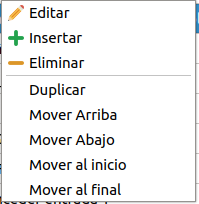
\includegraphics[scale=1, frame]{images/menu_contextual} 
\caption{Menu contextual de la lista de comandos}
\label{fig:menuContextual}
\end{figure}

En este menú se pueden realizar las siguientes acciones:

\begin{itemize}
\item \textbf{Editar:} Abre el \commandEditor{}, el cual permite personalizar el comando, posteriormente se profundiza en este tema.
\item \textbf{Insertar:} Inserta un comando nuevo en la ubicación seleccionada.
\item \textbf{Eliminar:} Elimina el comando seleccionado.
\item \textbf{Duplicar:} Duplica el comando seleccionado.
\item \textbf{Mover Arriba:} Mueve el comando seleccionado a la posición anterior.
\item \textbf{Mover Abajo:} Mueve el comando seleccionado a la siguiente posición.
\item \textbf{Mover al inicio:} Mueve el comando seleccionado a la primera posición.
\item \textbf{Mover al final:} Mueve el comando seleccionado a la última posición.
\end{itemize}

\subsection{Editor de comandos}
Los comandos son personalizables y se puede acceder a su configuración mediante el \commandEditor{}.

\begin{figure}[hbt!]\centering
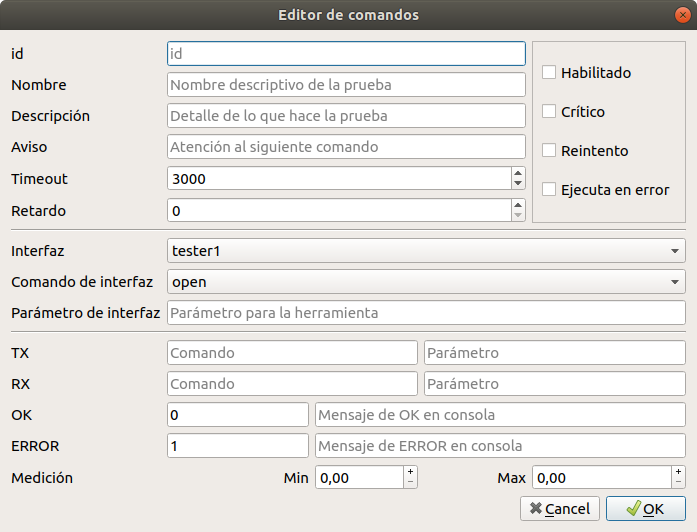
\includegraphics[scale=0.4, frame]{images/command_editor} 
\caption{Editor de comandos}
\label{fig:commandEditor}
\end{figure}

En la figura \ref{fig:commandEditor} se puede ver los campos que son personalizables en un comando, a continuación se detallan los mismos:

\begin{enumerate}
\item \textbf{id:} Cada comando tiene un identificador, el cual debe ser diferente del resto.
\item \textbf{Nombre:} Es el nombre que se muestra en el campo \textit{Prueba} de la lista de comandos.
\item \textbf{Descripción:} Es la descripción mas detallada de lo que hace el comando. Es visible en la \textit{lista de comandos} cuando se deja el puntero del ratón sobre alguna de las filas de la tabla.
\item \textbf{Aviso:} Mensaje que se mostrará en pantalla en el instante previo a la ejecución del comando, advirtiendo que se va a ejecutar el mismo.
\item \textbf{Timeout:} Es el tiempo que se puede esperar por una respuesta al comando. Expirado el tiempo se produce un error, exceptuando el caso de los comandos de demora, cuyo tiempo se configura en este campo.
\item \textbf{Retardo:} Es una demora que se produce en el instante anterior a la ejecución de un comando.
\item \textbf{Habilitado:} Activa o desactiva la ejecución del comando.
\item \textbf{Crítico:} Si un comando es crítico, la prueba finaliza en caso de producirse un error como respuesta a este comando.
\item \textbf{Reintento:} No implementado actualmente.
\item \textbf{Ejecuta en error:} Fuerza la ejecución de algún comando incluso si se produjo algún error crítico en pasos anteriores en la prueba.
\item \textbf{Interfaz:} Es el tipo de interfaz mediante la cual se ejecuta el comando.
\item \textbf{Comando de interfaz:} Es el comando que se ejecuta en la interfaz.
\item \textbf{Parámetro de interfaz:} Es el parámetro que se envía a la interfaz.
\item \textbf{TX:} Son los comandos y parámetros que se envían a través de la interfaz.
\item \textbf{RX:} Son los comandos y parámetros que se esperan recibir de la interfaz.
\item \textbf{OK:} Respuesta que se espera para considerar como exitosa la prueba correspondiente al comando. El campo de la derecha es un mensaje que se imprime en la consola cuando la prueba ha sido exitosa.
\item \textbf{ERROR:} Respuesta que se espera para considerar como fallida la prueba correspondiente al comando. El campo de la derecha es un mensaje que se imprime en la consola cuando la prueba ha sido fallida.
\item \textbf{Medición:} En caso de que el comando sea de medición, aquí se establecen los umbrales mínimo y máximo de medición, respectivamente.
\end{enumerate}

\subsection{Editor de interfaces}

\newpage

\section{Perfil de pruebas}
Con el propósito de dar flexibilidad y escalabilidad a \tarpuqJIGsw\, se creó el concepto del \textit{perfil de pruebas}. El perfil contiene toda la información mas relevante de un PCBA, como su código de inventario, el nombre del producto, el conjunto de pruebas que se necesitan realizar en el PCBA, y la información de las herramientas necesarias para llevar a cabo las pruebas. Los datos del perfil de pruebas están contenidos en un archivo JSON.

\subsection{Comandos}
Los \textbf{comandos} son el conjunto de pruebas que integran un perfil. Un comando es la acción, o conjunto de acciones que se llevan a cabo para ejecutar una prueba en concreto.

Los comandos necesitan de una interfaz para poder interactuar con los dispositivos que se van a probar.

\subsection{Interfaz} \label{defInterfaz}
La interfaz es la entidad mediante la cual se va a realizar una acción o se va a interactuar con algún dispositivo. Por ejemplo, la interfaz \textit{app} sirve para ejecutar acciones a nivel de aplicación, como ser una demora, cuadros de dialogo, etc.

\subsection{Abrir un perfil de pruebas} \label{loadProfile}
\begin{enumerate}
\item Desde la barra de menús, seleccionar \menu{Archivo>Abrir} o dando clic en su correspondiente icono en la barra de herramientas.
\item En el cuadro de dialogo que se abre, buscar la ruta donde se encuentra el archivo, seleccionarlo y dar clic en \keys{Abrir}.
\end{enumerate}

\subsection{Guardar un perfil de pruebas}
Hay dos opciones para guardar un perfil de pruebas, \textit{Guardar} y \textit{Guardar como}. La primera, permite guardar los cambios realizados en le perfil de pruebas actual. La segunda, abre un cuadro de dialogo donde se pide la ubicación para guardar el perfil con otro nombre.

Para guardar en el perfil actual:
\begin{enumerate}
\item Desde la barra de menús, seleccionar \menu{Archivo>Guardar} o dando clic en su correspondiente icono en la barra de herramientas.
\end{enumerate}

Para guardar en un nuevo perfil de pruebas:
\begin{enumerate}
\item Desde la barra de menús, seleccionar \menu{Archivo>Guardar como}.
\item En el cuadro de dialogo que se abre, buscar la ruta donde se deseas guardar el archivo, escribir un nombre y dar clic en \keys{Guardar}.
\end{enumerate}

\subsection{Apariencia de un perfil de pruebas}
Al cargar un perfil de pruebas, la interfaz principal de usuario muestra la información contenida en el perfil. Algo similar a lo que se muestra en la figura \ref{fig:mainLoaded}.

\begin{figure}[hbt!]\centering
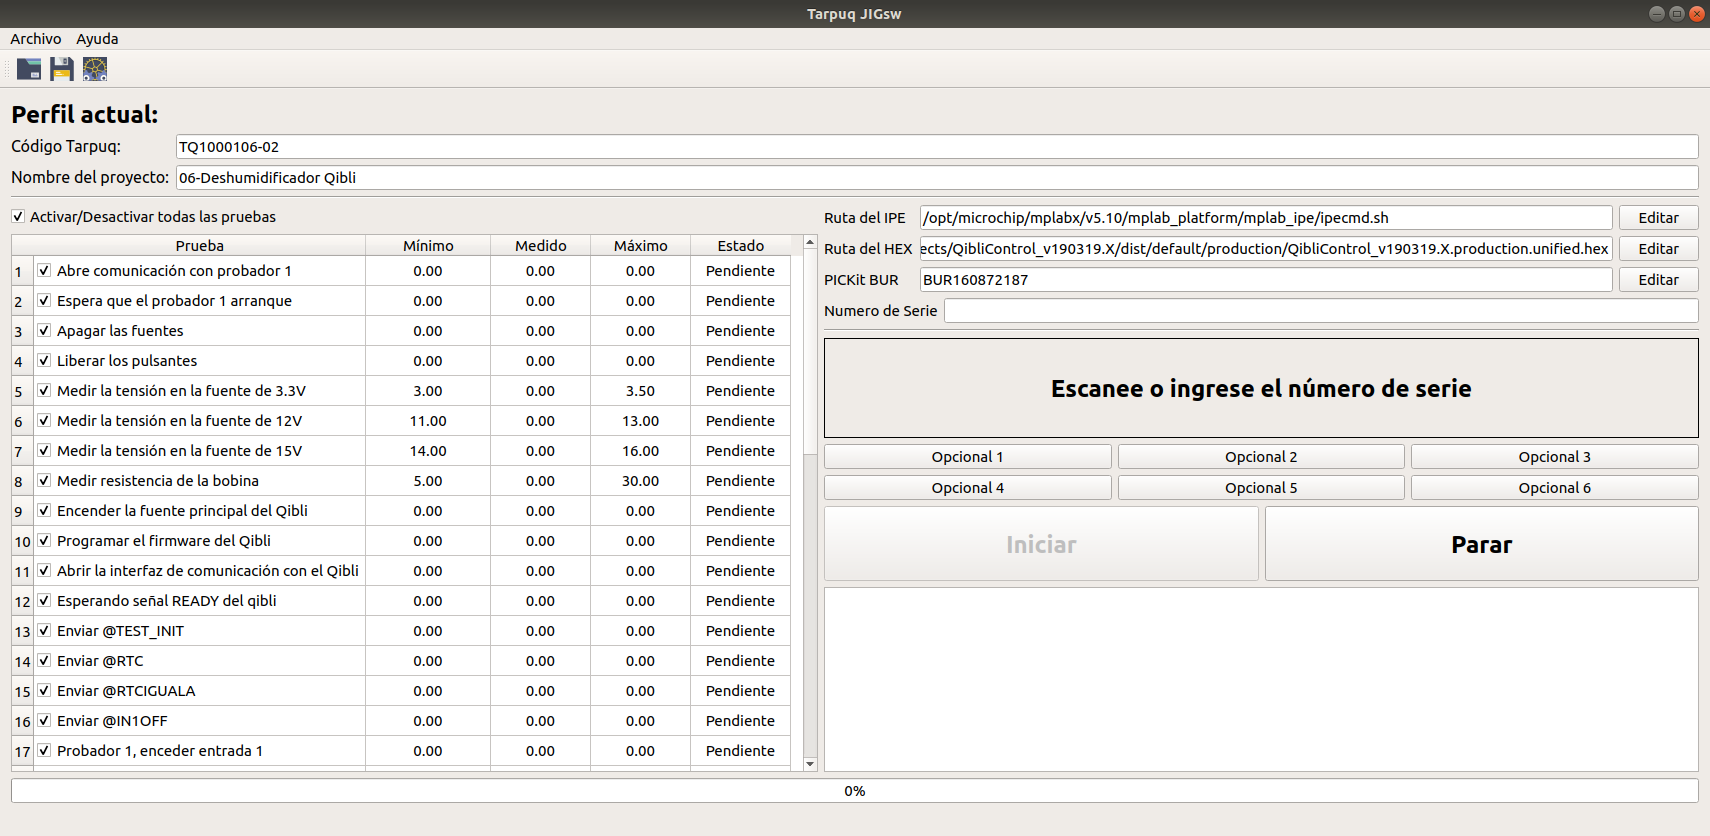
\includegraphics[width=\textwidth, frame]{images/main_profile_loaded} 
\caption{Apariencia de la interfaz de usuario al cargar un perfil.}
\label{fig:mainLoaded}
\end{figure}

En este punto es posible iniciar con el proceso de pruebas, o personalizar el perfil.

\newpage

\section{Ejecución del proceso de pruebas}
\subsection{Iniciar el proceso de pruebas}
Al momento de cargar un perfil, en la \textit{ventana principal} veremos que aparece un mensaje en el \textit{cuadro de mensajes} que dice ``Escanee o ingrese el número de serie'' indicando que debemos ingresar el número de serie del PCBA para poder continuar, esto es requisito.

En la \commandList{}, en el campo Prueba, es posible activar o desactivar las pruebas que se ejecutarán en el proceso, mediante la casilla de verificación de cada comando. Debe realizarse este paso previo al inicio del proceso, de ser requerido.

Una vez ingresado el número de serie, nos muestra el mensaje ``Pulse 'Iniciar' para empezar'', esto nos indica que se puede iniciar el proceso de pruebas dando clic en \textit{Iniciar} o presionando la tecla \textit{Espacio}, como se muestra en la figura \ref{fig:snReaded}.

\begin{figure}[hbt!]\centering
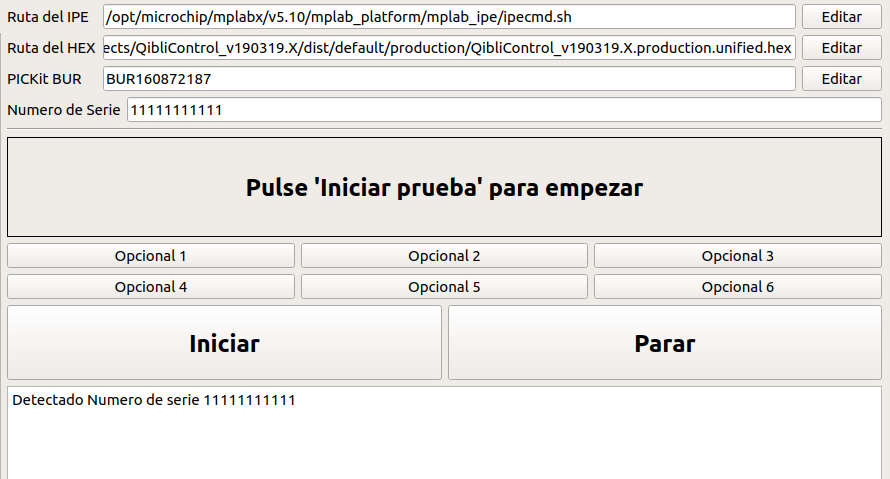
\includegraphics[width=\textwidth, frame]{images/serial_number_readed} 
\caption{Ingresado número de serie}
\label{fig:snReaded}
\end{figure}

Por lo tanto, para iniciar el proceso de pruebas, se pueden seguir los siguientes pasos:

\begin{enumerate}
\item Tener cargado el perfil de pruebas, de no estarlo, seguir los pasos indicados en la sección \ref{loadProfile}.
\item Verificar que las pruebas activadas/desactivadas en el campo Prueba de la \commandList\ correspondan a las requeridas en el proceso.
\item Ingresar el número de serie en su respectivo campo, y presionar la tecla \keys{\enter}.
\item Colocar el PCBA en su respectivo JIG, respetando las debidas indicaciones del \textit{instructivo de trabajo}.
\item Dar clic en el botón \keys{Iniciar}, o presionar la tecla \keys{\SPACE} cuando esté listo.
\item Esperar que el proceso finalice.
\end{enumerate}

\subsection{Posibles resultados}
Cuando se \textit{Inicia} el proceso de pruebas, el programa verifica si la prueba está activada. Si la prueba se encuentra desactivada, el programa salta al siguiente comando y pone el estado \textcolor[rgb]{0,0,1}{``Salta''}. Cuando la prueba concluye exitosamente, el estado se pone en \textcolor[rgb]{0,1,0}{``OK''}. Mientras que si hubo algún error, el estado se pone en \textcolor[rgb]{1,0,0}{``ERROR''}. Un ejemplo de estos estados se puede ver en la figura \ref{fig:runningTest1}.

\begin{figure}[hbt!]\centering
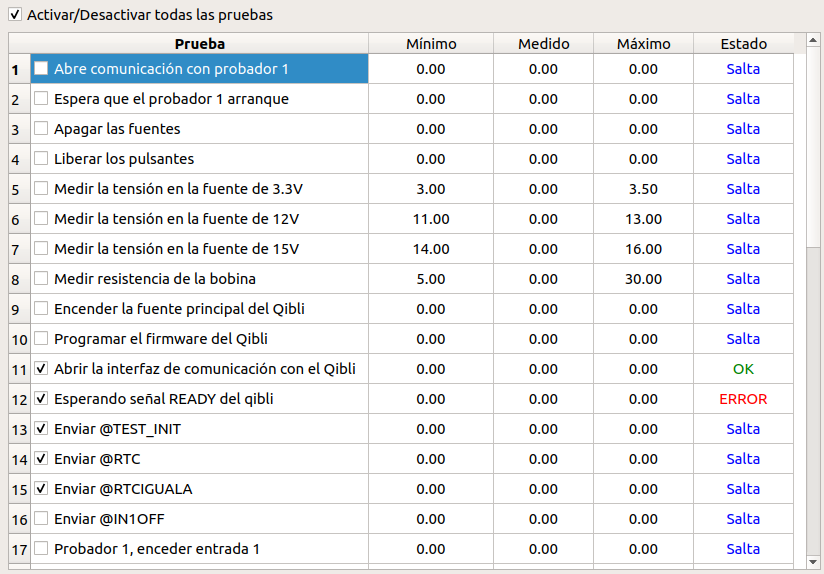
\includegraphics[width=\textwidth, frame]{images/running_test_error_1} 
\caption{Estados de las pruebas}
\label{fig:runningTest1}
\end{figure}

Es suficiente con que se produzca un error, y el proceso de pruebas queda invalidado y devuelve el mensaje de que el PCBA ``NO PASA'' las pruebas, como se puede ver en la figura \ref{fig:runningTest2}, con fondo rojo en el cuadro de mensajes. Una prueba exitosa devuelve el mensaje ``PASA'' en fondo verde.

\begin{figure}[hbt!]\centering
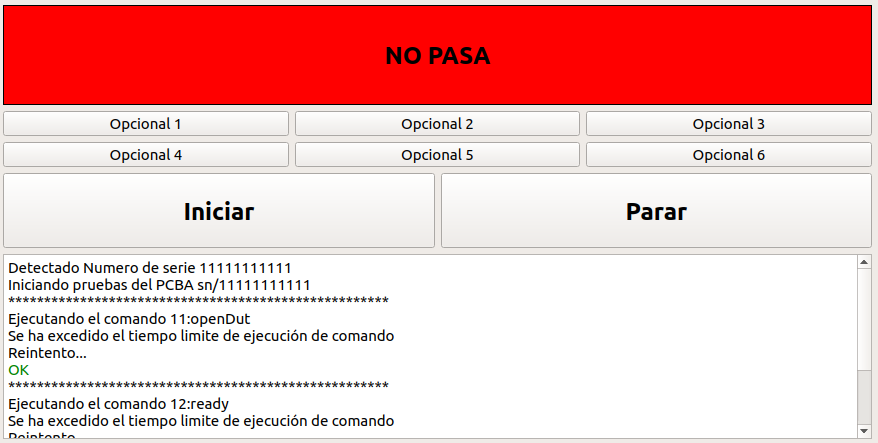
\includegraphics[width=\textwidth, frame]{images/running_test_error_2} 
\caption{Resultado final de una prueba con error}
\label{fig:runningTest2}
\end{figure}

\newpage

\subsection{Registro de las pruebas}
\tarpuqJIGsw{} registra los detalles de las pruebas en la base de datos. Los reportes de fallos pueden ser creados con la aplicación \emph{AppReporteEquipos} y en ésta se puede identificar varios campos importantes:

Para todos los casos, se registran los siguientes datos:

\begin{enumerate}
\item Nombre del producto en pruebas.
\item Número de serie del equipo
\item Resultado de la prueba.
\item Lista con los fallos detectados.
\item Lista con la descripción de los fallos.
\item Fecha y hora del registro.
\item Tiempo total transcurrido en la ejecución de la prueba.
\end{enumerate}

Cuando la prueba finaliza correctamente, sin fallos, se registra un mensaje de ``ok''. Cuando alguno de los comandos detecta algún error, se registra el indice del comando con su id, y el mensaje de fallo configurado en el \commandEditor{}.

\section{Personalizar el perfil de pruebas}
\subsection{Datos del PCBA}
Para cambiar el Código Tarpuq y el Nombre del Producto al que pertenece el PCBA en pruebas, hay que dar clic en el botón \keys{Editar} correspondiente a cada campo.

\subsection{Datos para la programación de Firmware}
En la \textit{ventana principal} hay tres campos que nos permiten configurar los parámetros necesarios para programar un Firmware en el PCBA. Aquí encontramos la ruta hacia la aplicación que controla el PICKit, también conocida como \emph{ipecmd.sh}. La ruta del archivo hexadecimal con el Firmware que será programado. Y por último el número de serie del PICKit que se usará en el proceso.

\begin{figure}[hbt!]\centering
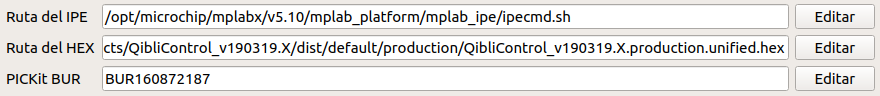
\includegraphics[width=\textwidth, frame]{images/pickit_data} 
\caption{Parámetros para el PICKit}
\label{fig:pickitData}
\end{figure}

Para cambiar estos parámetros hay que dar clic en el botón \keys{Editar} que corresponde a cada campo.

\subsubsection{Ruta del IPE}
\begin{enumerate}
\item Dar clic en el botón \keys{Editar} del campo \emph{Ruta del IPE}
\item En el cuadro de diálogo que se abre, buscar la ubicación de \emph{ipecmd.sh}, por defecto se encuentra en: \\
\directory{/opt/microchip/mplabx/vX.YY/mplab\_platform/\\
mplab\_ipe/ipecmd.sh}
\item Dar clic en \keys{Abrir}
\end{enumerate}

\subsubsection{Ruta del HEX}
\begin{enumerate}
\item Dar clic en el botón \keys{Editar} del campo \emph{Ruta del HEX}
\item En el cuadro de diálogo que se abre, buscar la ubicación del archivo hexadecimal que contiene el Firmware. Siempre será un archivo de extensión \emph{*.hex}.
\item Dar clic en \keys{Abrir}
\end{enumerate}

\subsubsection{PICKit BUR}
\begin{enumerate}
\item Dar clic en el botón \keys{Editar} del campo \emph{PICKit BUR}
\item Escribir el número de serie del PICKit, el cual puede encontrarse en su parte posterior, o a través de la aplicación MPLAB X IPE (marcado en el recuadro rojo en la figura \ref{fig:pickitBur}). Siempre es un código que empieza con BUR.
\item Presionar \keys{\enter} para guardar el cambio.

\begin{figure}[hbt!]\centering
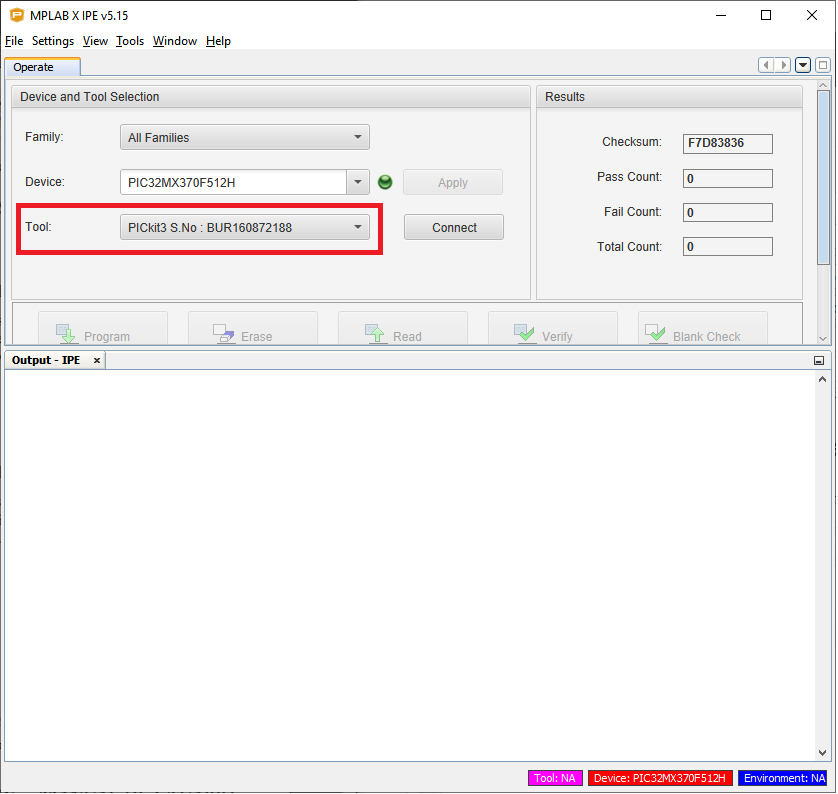
\includegraphics[width=\textwidth, frame]{images/pickit_bur} 
\caption{Número de serie del PICKit}
\label{fig:pickitBur}
\end{figure}

\end{enumerate}

\subsection{Comandos}
Como se vio en la sección \ref{ref:commandList}, se puede manipular las posiciones de los comandos mediante el menú contextual de la \commandList{}. También es posible editar las acciones y los datos de los comandos mediante el \commandEditor{}.

\subsection{Interfaz}
En la sección \ref{defInterfaz} se definió lo que es una interfaz. Ahora se profundiza sobre el manejo de las interfaces.

Por defecto se identifican 3 interfaces:
\begin{itemize}[noitemsep]
\item app
\item dut
\item pickit
\end{itemize}

Se puede utilizar los siguientes tipos de interfaz:
\begin{itemize}[noitemsep]
\item app
\item plugin
\item tty
\item usb
\end{itemize}

La interfaz \textit{app} es del tipo \textit{app}, es decir, no tiene ningún puerto específico para comunicación. La interfaz \textit{dut} es del tipo \textit{tty}, ya que utiliza un puerto de comunicación serial (normalmente un adaptador USB-Serial) para interactuar con el dispositivo bajo pruebas. La interfaz \textit{pickit} es del tipo \textit{usb}, ya que el pickit es un dispositivo que está conectado a un puerto USB.

\medskip

\begin{leftbar}
Las interfaces podrán ser creadas, configuradas, eliminadas, mediante un gestor de interfaces (disponible en versiones posteriores).
\end{leftbar}

Para brindar mayor flexibilidad al proceso de pruebas, se puede crear interfaces adicionales del tipo \textit{tty}. Normalmente estas interfaces son para controlar dispositivos auxiliares que pueden servir para encender o apagar equipos, para medir tensiones, para medir variables patrón, etc. Estas interfaces pueden nombrarse como \textit{tester1}, \textit{tester2}, etc.

\subsubsection{Comando de interfaz}
Para interactuar con los dispositivos a través de las interfaces, se utiliza los \textit{comandos de interfaz}. Hay ciertos comandos que son inherentes a cada interfaz. La interfaz \textit{app} responde a los comandos \textit{dialog, deadtime, loraserverapi, end}. Las interfaces \textit{tty} responden a los comandos \textit{open, close, usartXfer}. La interfaz \textit{pickit} responde al comando \textit{program}.

\subsubsection{Argumentos de interfaz}
Son los argumentos que serán anexados al comando de la interfaz. Por ejemplo el comando \textit{app:dialog} donde el parámetro es el mensaje que se mostrará en el cuadro de diálogo que aparecerá en pantalla. O los argumentos para la ejecución de un proceso externo.

\subsection{Comandos TX y RX}
Estos comandos son específicos de las interfaces tipo \textit{tty}, sirven para recibir y enviar comandos desde y hacia el dispositivo conectado a la interfaz. 

Los comandos son cadenas de texto ASCII terminadas en $\left\langle CR \right\rangle \left\langle LF \right\rangle$ y en caso de existir parámetros, estos se anteponen al final de cadena. Los parámetros pueden ser valores fijos o comodines. Estas variables comodín se utilizan con \% y posteriormente se profundizará sobre ellas.

Las mecánicas de interacción son las siguientes:

\subsubsection{Envío de comando síncrono con espera de respuesta OK o ERROR}
Útil cuando se necesita enviar un comando a un dispositivo, y no se requiere mayor respuesta de su parte que un mensaje de confirmación, el cual puede indicar un estado de OK o de ERROR, dependiendo de la acción que desempeñe el comando.

Formato de las tramas:
\\
\begin{table}[H]
\small\centering
\begin{tabular}{|c|l|}
\hline 
TX & [CMDtx] $\left\langle CR \right\rangle \left\langle LF \right\rangle$ \\ 
\hline 
RX & [ECO] $\left\langle CR \right\rangle \left\langle LF \right\rangle$ \\
   & [ANS] $\left\langle CR \right\rangle \left\langle LF \right\rangle$ \\ 
\hline 
\end{tabular} 
\end{table}

Donde CMDtx es la cadena del campo Comando en TX. ECO es el eco del comando que se envío al equipo. ANS es la respuesta que el comando produce, la cual puede tomar el valor de 0 ó 1, para OK o ERROR, respectivamente.

Ejemplo: Un dispositivo auxiliar puede encender o apagar una fuente mediante el comando \textit{powerOn} y \textit{powerOff} respectivamente, responde con 0 si la acción se llevó a cabo exitosamente, o con 1 si hubo algún error. La configuración sería como en la figura \ref{fig:commands1}.

\begin{figure}[H]\centering
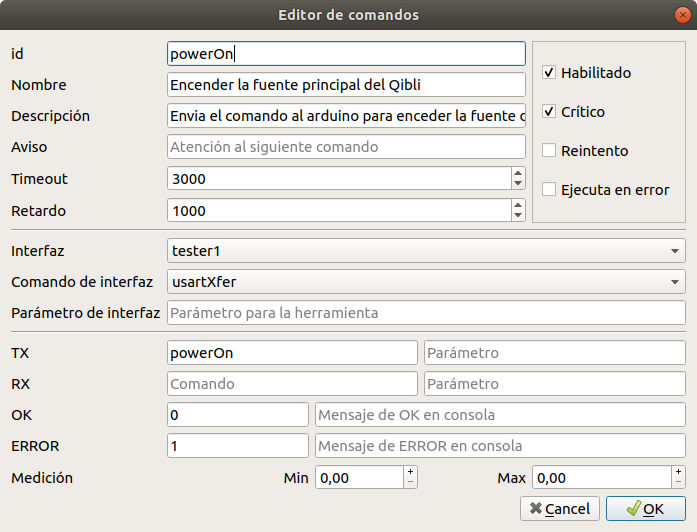
\includegraphics[scale=0.4, frame]{images/commands1} 
\caption{Comando síncrono con espera de OK o ERROR}
\label{fig:commands1}
\end{figure}

\subsubsection{Envío de comando síncrono con parámetro y espera de respuesta OK o ERROR}
Igual que el caso anterior, sólo que ahora se envía un parámetro en conjunto con el comando.

Formato de las tramas:
\\
\begin{table}[H]
\small\centering
\begin{tabular}{|c|l|}
\hline 
TX & [CMDtx][PARtx] $\left\langle CR \right\rangle \left\langle LF \right\rangle$ \\ 
\hline 
RX & [ECO CMDtx PARtx] $\left\langle CR \right\rangle \left\langle LF \right\rangle$ \\
 & [ANS] $\left\langle CR \right\rangle \left\langle LF \right\rangle$ \\ 
\hline
\end{tabular} 
\end{table}

Donde CMDtx y PARtx son las cadenas de los campo Comando y Parámetro en TX, respectivamente. ECO CMDtx PARtx es el eco del comando y parámetro que se envío al equipo. ANS es la respuesta que el comando produce, la cual puede tomar el valor de 0 ó 1, para OK o ERROR, respectivamente.

Ejemplo: Un dispositivo puede poner el estado de un pin en 1 o 0, mediante un comando pb1. El estado se refleja del parámetro que se envía el cual puede ser 1 o 0 para encender o apagar respectivamente. La configuración sería como en la figura \ref{fig:commands2}.

\begin{figure}[H]\centering
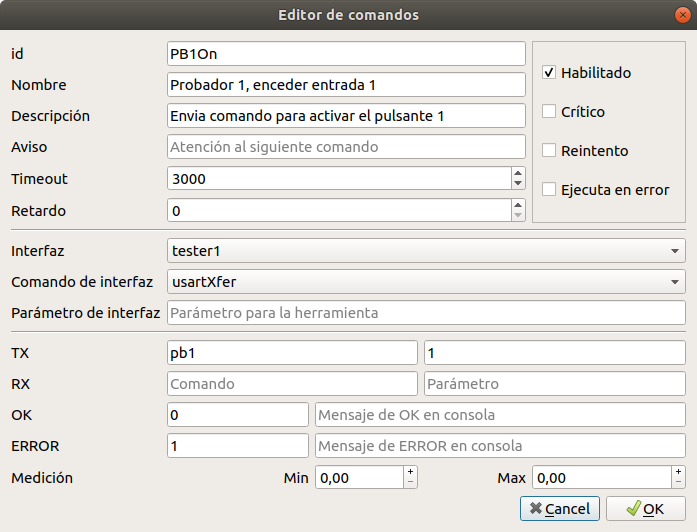
\includegraphics[scale=0.4, frame]{images/commands2} 
\caption{Comando síncrono con parámetro y espera de OK o ERROR}
\label{fig:commands2}
\end{figure}

\subsubsection{Envío de comando síncrono que espera la recepción de un parámetro, con detección de OK o ERROR} \label{txCmd&rxPar}
Hay comandos que no requieren el envío de un parámetro y devuelven una respuesta de interés, aparte del habitual OK y ERROR.

Formato de las tramas:
\\
\begin{table}[H]
\small\centering
\begin{tabular}{|c|l|}
\hline 
TX & [CMDtx] $\left\langle CR \right\rangle \left\langle LF \right\rangle$ \\
\hline 
RX & [ECO CMDtx] $\left\langle CR \right\rangle \left\langle LF \right\rangle$ \\ 
 & [PARrx] $\left\langle CR \right\rangle \left\langle LF \right\rangle$ \\
 & [ANS] $\left\langle CR \right\rangle \left\langle LF \right\rangle$ \\ 
\hline
\end{tabular} 
\end{table}

Donde CMDtx es la cadena del campo Comando en TX. ECO CMDtx es el eco del comando que se envío al equipo. PARrx es la cadena del campo Parámetro en RX y es la respuesta de interés. ANS es la respuesta que el comando produce, la cual puede tomar el valor de 0 ó 1, para OK o ERROR, respectivamente.

Ejemplo: Se necesita leer un valor de referencia desde un dispositivo que mide la temperatura ambiente de un habitación. Este recibe como comando \textit{t} y devuelve la temperatura, la cual es almacenada en un comodín llamado \%reference. Finaliza con 0 o 1 en caso de OK o ERROR. La configuración sería como en la figura \ref{fig:commands3}.

\begin{figure}[H]\centering
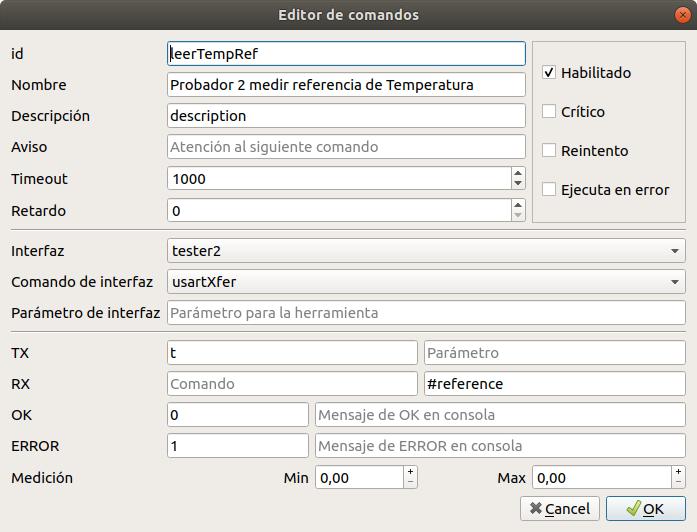
\includegraphics[scale=0.4, frame]{images/commands3} 
\caption{Comando síncrono con espera de respuesta y confirmación OK o ERROR}
\label{fig:commands3}
\end{figure}

\subsubsection{Envío de comando síncrono con parámetro que espera la recepción de un parámetro, con detección de OK o ERROR}
Similar al caso anterior, solo que ahora si se envía un parámetro.

Formato de las tramas:
\\
\begin{table}[H]
\small\centering
\begin{tabular}{|c|l|}
\hline
TX & [CMDtx][PARtx] $\left\langle CR \right\rangle \left\langle LF \right\rangle$ \\
\hline 
RX & [ECO CMDtx PARtx] $\left\langle CR \right\rangle \left\langle LF \right\rangle$ \\
   & [PARrx] $\left\langle CR \right\rangle \left\langle LF \right\rangle$ \\
   & [ANS] $\left\langle CR \right\rangle \left\langle LF \right\rangle$ \\ 
\hline
\end{tabular} 
\end{table}

Donde CMDtx y PARtx son las cadenas de los campos Comando y Parámetro en TX, respectivamente. ECO CMDtx PARtx es el eco del comando que se envío al equipo. PARrx es la cadena del campo Parámetro en RX y es la respuesta de interés. ANS es la respuesta que el comando produce, la cual puede tomar el valor de 0 ó 1, para OK o ERROR, respectivamente.

Ejemplo: Se necesita medir el voltaje de una fuente configurada como fuente 1, mediante un comando \textit{testSource} y el parámetro 1 para indicar que es la fuente 1. El resultado se guarda en la variable \%measure. La configuración sería como en la figura \ref{fig:commands4}

\begin{figure}[H]\centering
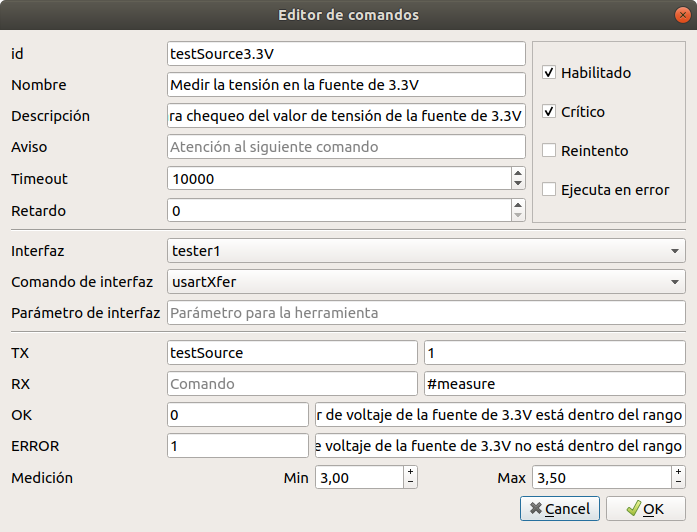
\includegraphics[scale=0.4, frame]{images/commands4} 
\caption{Comando síncrono con parámetro y  espera de respuesta, confirmación OK o ERROR}
\label{fig:commands4}
\end{figure}

\subsubsection{Recepción asíncrona de un comando}
Espera por la recepción de un comando el cual llegará de forma asíncrona.

Formato de la trama:
\\
\begin{table}[H]
\small\centering
\begin{tabular}{|c|l|}
\hline 
RX & [CMDrx] $\left\langle CR \right\rangle \left\langle LF \right\rangle$ \\ 
\hline
\end{tabular}
\end{table}

Donde CMDrx es la cadena del campo Comando en RX. Es lo que se espera recibir desde el dispositivo.

Ejemplo: Un dispositivo envía un mensaje @Ready una vez que ha terminado su secuencia de inicio y de esta forma indica que está listo para procesar comandos. La configuración sería como en la figura \ref{fig:commands5}.

\begin{figure}[H]\centering
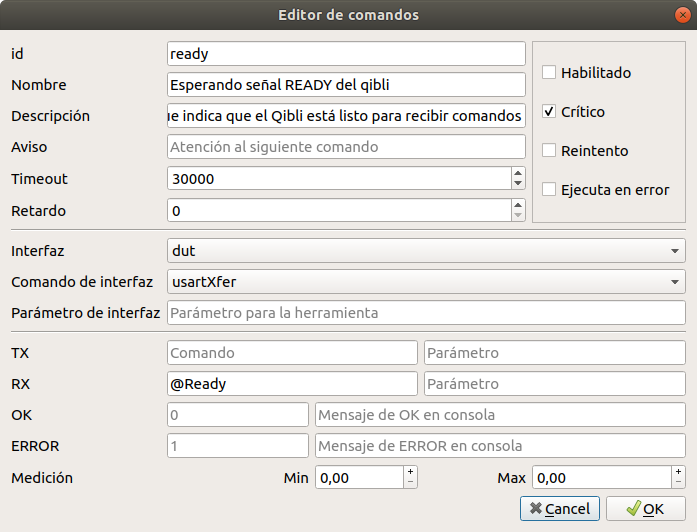
\includegraphics[scale=0.4, frame]{images/commands5} 
\caption{Recepción asíncrona de un comando.}
\label{fig:commands5}
\end{figure}

En la figura \ref{fig:commands5} se puede ver que en estos casos, solo es necesario configurar el comando que se espera recibir por parte de algún dispositivo, el comando llega sin la necesidad de enviar alguna petición. Por lo tanto no es necesaria una confirmación por parte del dispositivo.

\subsubsection{Recepción asíncrona de un comando con parámetro}
Igual que en el caso anterior, pero ahora el comando viene acompañado de un parámetro que necesita ser leído.

Formato de la trama:
\\
\begin{table}[H]
\small\centering
\begin{tabular}{|c|l|}
\hline 
RX & [CMDrx][PARrx] $\left\langle CR \right\rangle \left\langle LF \right\rangle$ \\ 
\hline
\end{tabular}
\end{table}

Donde CMDrx y PARrx son las cadenas de los campos Comando y Parámetro en RX, respectivamente. Es lo que se espera recibir desde el dispositivo.

Ejemplo: Un dispositivo envía la hora después de su arranque con el siguiente formato RTC: dd/MM/yyyy HH:mm:ss, es necesario leer esa hora y verificar que sea igual a la hora del sistema. En este caso se puede usar el comodín \%D para almacenar el parámetro. La configuración sería como en la figura \ref{fig:commands6}.

\begin{figure}[H]\centering
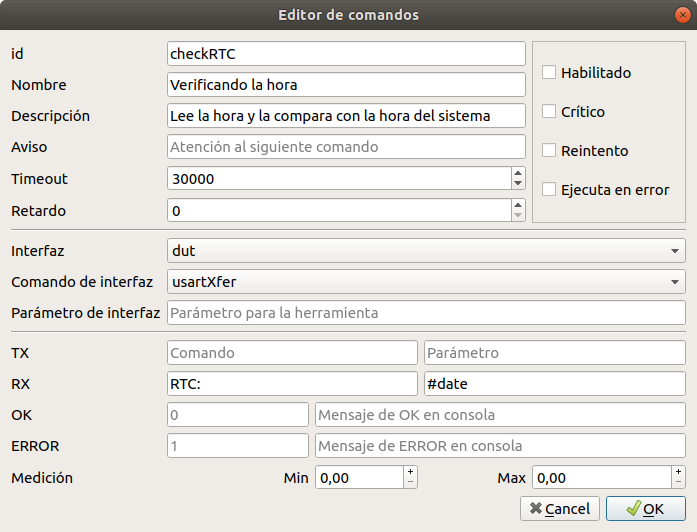
\includegraphics[scale=0.4, frame]{images/commands6} 
\caption{Recepción asíncrona de un comando con parámetro.}
\label{fig:commands6}
\end{figure}

\subsection{Mediciones}
Algunas pruebas requieren la medición de ciertas magnitudes del PCBA, como ser voltaje, resistencia, corriente, entre otras. Se puede crear comandos que permitan medir estos valores y compararlos dentro de un umbral para validar su magnitud. El rango está delimitado por el valor mínimo y máximo del comando, estos valores son configurables. No todos los comandos soportan medición. Aquellos que no requieran de mediciones, ignorarán estos parámetros.

\subsection{Comodines:}
Los comodines sirven para enviar y recibir ciertos valores que pueden cambiar en el tiempo, por ejemplo: El número de serie del equipo, la fecha, una medición, etc.

Los comodines predeterminados son:
\begin{itemize}
\item \textbf{\%D:} Sirve para enviar la fecha actual en un comando TX, o para comparar la fecha actual en un comando RX.
\item \textbf{\%measure:} Usada como parámetro RX, sirve para identificar que la respuesta entregada por el equipo es una medición y que por lo tanto debe ser tratada como tal.
\item \textbf{\%serialNumber:} Sirve para enviar el número de serie del dispositivo en caso de ser usada como parámetro TX, o compara el valor con el número de serie actual en caso de ser usada como parámetro RX.
\end{itemize}

En el ejemplo del numeral \ref{txCmd&rxPar} de comandos TX y RX, se vio que se utilizó el comodín \%reference, el cual no está definido como predeterminado (es decir que podría tener cualquier otro nombre, siempre iniciando con \%). Lo importante de los comodines es que almacenan el dato en memoria, y mantiene su valor durante toda la prueba. Por lo tanto se puede leer una referencia de un dispositivo, almacenarlo en un comodín llamado \%foo e inmediatamente enviarlo como parámetro a otro dispositivo, agregando a \%foo como argumento TX del comando a ser enviado.

\end{document}
